\section{Bonus DTW}

\begin{frame}
  \centering
  {\Large Optimal Square Detection  Over General Alphabets}

  \bigskip
  {\large SPIRE'22}\\
  \bigskip
  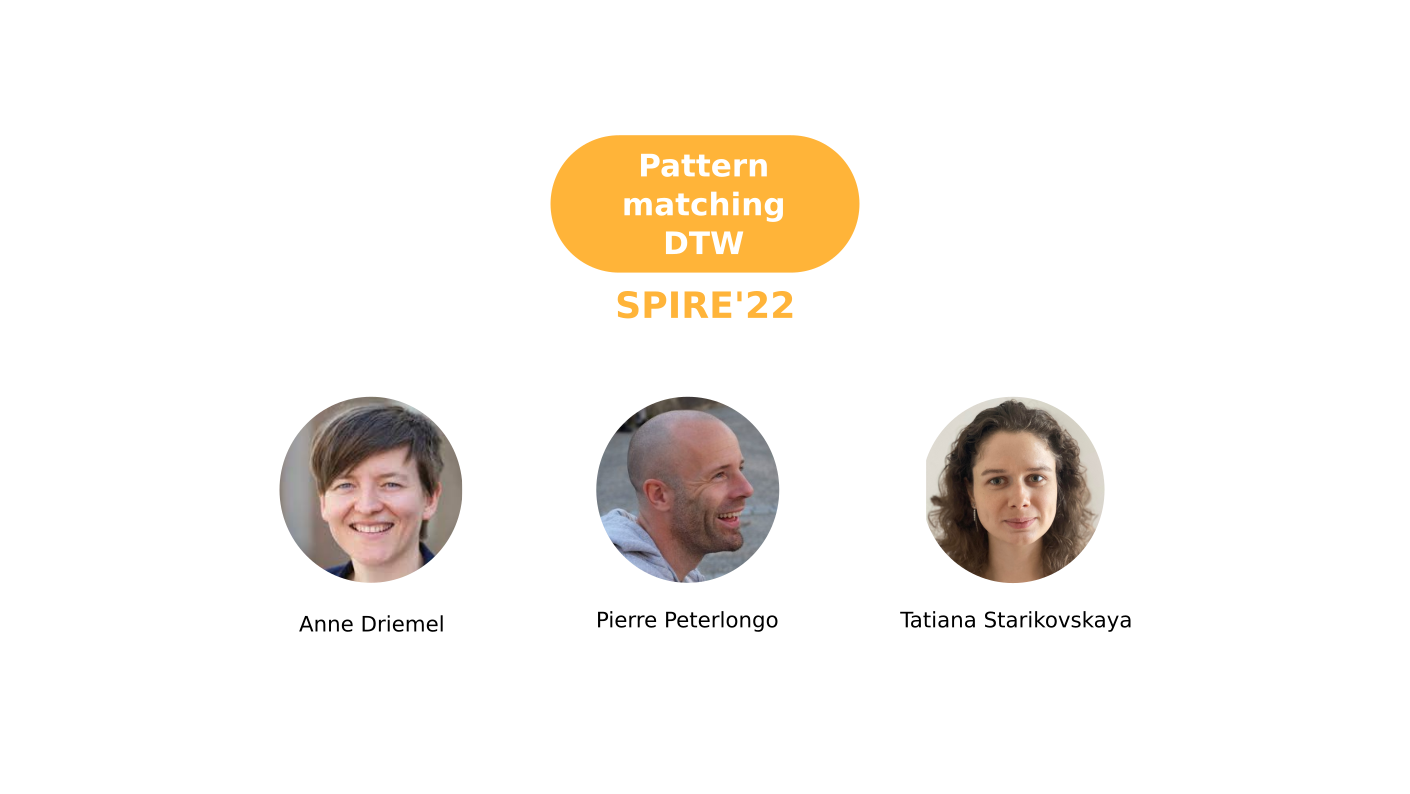
\includegraphics{pictures/mindmap/dtw.png}

  \bigskip
  Anne Driemel, Pierre Peterlongo, Tatiana Starikovskaya
\end{frame}

\begin{frame}{Formal definition of $\dtw(X,Y)$ and dynamic programming}

  \begin{columns}
  \column{0.45\textwidth}
  \newcommand{\dtwgrid}[2]{% height width 
\foreach \i in {0,...,#1} {
	\foreach \j in {0,...,#2} {
		\filldraw[black] (\i , \j) circle (2pt);
		\ifthenelse{ \not \equal{#2}{\j}}{ 
			\draw[->] ($(\i , \j+0.9)$) -- ($(\i , \j+0.1)$);
		}{}
		\ifthenelse{ \not \equal{#1}{\i}}{
  			\draw[->] ($(\i +0.1 , \j)$) -- ($(\i +0.9 , \j)$);
		}{}
		\ifthenelse{\not\equal{#1}{\i} \and \not \equal{#2}{\j}}{%
  			\draw[->] ($(\i +0.1 , \j + 0.9)$) -- ($(\i +0.9, \j + 0.1)$);
  		}{}
	}
}
}

\newcommand{\dtwarrow}[2]{%
\draw[->,line width=0.3mm,red] #1 -- #2;
}

  \begin{figure}
      \beamermathcolor{black}
      \centering
      \begin{tikzpicture}[scale=0.8, every node/.style={scale=1.2}]
      \dtwgrid{5}{2}
  
      \foreach \i in {1,...,6} {
          \node at ($(\i-1, 2.8)$) {\tiny{$X[\i]$}};
      }
      \foreach \j in {1,...,3} {
          \node at ($(-1.2, 3 -\j )$) {\tiny{$Y[\j]$}};
      }
  
      \foreach \x[count=\i] in {C,A,A,A,G,G} {
          \node at ($(\i-1 , 2.3)$) {\textcolor{black}{\tiny{\x}}};
      }
      \foreach \y[count=\j] in {A,T,G} {
          \node at ($(-0.5, 3 -\j )$) {\textcolor{black}{\tiny{\y}}};
      }
  
  
      \only<2->{
          \dtwarrow{(0.1,2)}{(0.9,2)}
          \dtwarrow{(3.1,1.9)}{(3.9,1.1)}
          \dtwarrow{(1.1,2)}{(1.9,2)}
          \dtwarrow{(2.1,2)}{(2.9,2)}
          \dtwarrow{(4,0.9)}{(4,0.1)}
          \dtwarrow{(4.1,0)}{(4.9,0)}
          \node at (5,-0.3) {\bred{$\pi$}};
      }
  
      \end{tikzpicture}
  \end{figure}
  \column{0.45\textwidth}
  \centering
  \only<3>{
  $\text{cost}(\pi) = \sum_{(i,\ j)\in \pi} d(X[i],Y[j])$\\
  \vspace{0.5cm}
  $\dtw(X,Y) = \min_{\pi} \text{cost}(\pi)$\\
  \vspace{0.5cm}
  {\small s.t. $\pi$ goes from top left to bottom right.}}
  \end{columns}
  \pause %grid definition 
  \pause %draw the path
  \pause
  
  \bigskip
  
  
  \only<4|handout:0>{
  \begin{exampleblock}{Path correspondance to alignment}
  \center
  \begin{figure}
  %\missingfigure{Under construction...}
  \centering
  \begin{tikzpicture}[scale=0.7, every node/.style={scale=1}]
  \foreach \x[count=\i] in {C,A,A,A,G,G} {
      \node at ($(\i, 1)$) {\small{\x}};
  }
  \foreach \y[count=\j] in {A,T,G} {
      \node at ($(0.5+\j*1.5, 0)$) {\small{\y}};
  }
  % align A
  \fill[myblue!25] (2, 0.25) -- (2,0.75) -- (4,0.75) -- (2.1,0.25) -- cycle;
  % align G
  \fill[myblue!25] (5, 0.25) -- (5,0.75) -- (6,0.75) -- (5.1,0.25) -- cycle;
  %draw misalignment
  \draw[dashed,red] (1.75, 0.25) -- (1,0.75);
  \draw[dashed,red] (3.5, 0.25) -- (5,0.75);
  \end{tikzpicture}
  \end{figure}
  \vfill
  $\dtw($CAAAG$,$ATG$)=2$
  \end{exampleblock}}
  
  \only<5->{
  
  \btheme{Dynamic Programming solution}\\
  \smallskip
  $D$ a matrix of size $(M+1)(N+1)$ such that $D[i,j]=\dtw(X[1..i],Y[1..j])$\pause
  \bigskip
  
  \btheme{Initialization}~~~$D[0,0]= 0$ and for all $(i,j)$, $D[0,j]=D[i,0]=+\infty$.\\
  \pause
  \bigskip
  \btheme{Recurrence} ~~~ 
      $D[i,j] = \min\{$\beamermathcolor{black}
          $\underbrace{\mathcolor{black!30!blue}{D[i-1,j-1]}}_\text{top-left},
          \underbrace{\mathcolor{black!30!blue}{D[i-1,j]}}_\text{top},
          \underbrace{\mathcolor{black!30!blue}{D[i,j-1]}}_\text{left}$
      $\mathcolor{black!30!blue}{\}+ d(X[i], Y[j])}$.
  }
  
  \end{frame}
  

\begin{frame}{}

  \textbf{Our contributions:}\\
  For $T$ and $P$ two strings, $|T|=N$ and  $|P|=M$, $|\RLE(T)|=n$ and  $|\RLE(P)|=m$.
  Pattern matching under DTW distance:
  \begin{itemize}
  \item $\Oh(Nm+nM)$-time general algorithm which can for an integer distance, compute all values bellow $k$ in $\Oh(nmk)$-time. \pause
  \item Toy implementation available on github.\pause
  \item An $\Oh(L^{\eps})$-approximation, for any $0 < \eps < 1$, in  $\Oh(L^{1-\eps} \cdot mn \log^3 L)$-time with $L=\max(N,M)$.\pause
  \item (A $\Oh(n+m)$-time algorithm for $k=1$.)\pause
  \end{itemize}
  
  
  \textbf{Open questions:}
  \begin{itemize}
  \item Is a $\Oh(k(n+m))$-time algorithm possible? \pause
  \item Can those improvements benefit applications ?\pause
  \end{itemize}
  \end{frame}


\begin{frame}{Experiments: visualization on simulated data}
  Problem: How to design a protocol that isn't biased towards ED ?\\
  Model to illustrate the impact of homopolymers on ED.
  \begin{center}
    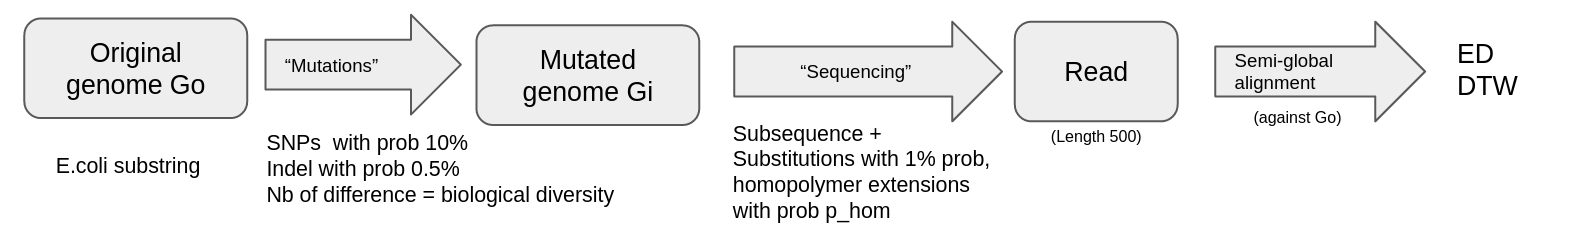
\includegraphics[scale=0.2]{figures/pipeline.png}
  \end{center}
  \vspace{-0.5cm}
  \begin{columns}
    \column{0.3\textwidth}
    
    We compare the values of the two distances as the probability of extending homopolymers increases.
    
    \column{0.5\textwidth}
    \begin{center}
      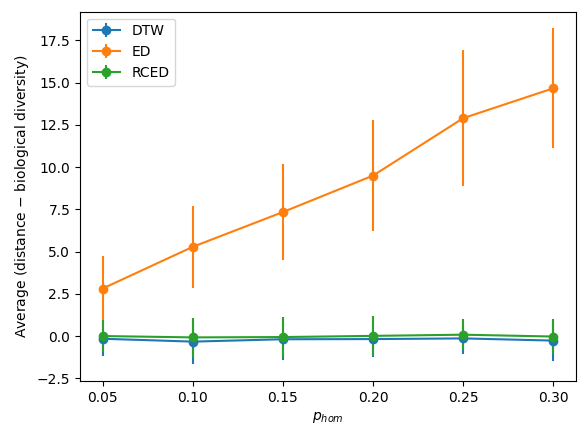
\includegraphics[scale=0.4]{figures/ecoli_10kb_N_100_fixed_ID_0.0005.png}
    \end{center}
  \end{columns}
\end{frame}


\begin{frame}{Comparison to the edit distance}
  \beamermathcolor{black}
  \[
  D[i,j] = {\min\{
  \underbrace{D[i-1,j-1]}_\text{top-left},
  \underbrace{D[i-1,j]}_\text{top},
  \underbrace{D[i,j-1]}_\text{left}
  \} \mathcolor{red}{+ d(X[i], Y[j])}
  }
      \]
  
  \[
  ED[i,j] = {\min\{
  \underbrace{ED[i-1,j-1]}_\text{top-left} \mathcolor{red}{+ d(X[i], Y[j])},
  \underbrace{ED[i-1,j]}_\text{top} \mathcolor{red}{+1},
  \underbrace{ED[i,j-1]}_\text{left} \mathcolor{red}{+1}
  \}
  }
      \]
  
  \pause
  
  \only<2-3|handout:0>{
  \begin{exampleblock}{DTW vs ED}
  $\ed(AAAA\mathcolor{myblue}{T}G,AA\mathcolor{myblue}{T}C)=3$ whereas $\dtw(AAAA\mathcolor{myblue}{T}G,AA\mathcolor{myblue}{T}C)=1$.\\
  $\dtw(AAAA\mathcolor{myblue}{T}G,AA\mathcolor{myblue}{T}CCC)=3$
  \end{exampleblock} 
  
  \only<3>{$\Rightarrow$ Compresses runs of matching letters!}
  }

  \only<4>{
    \begin{center}
      
\begin{center}
\footnotesize
\resizebox{0.8\textwidth}{!}{
\begin{tabular}{|cc||cc|cccc|c|cc|c|cccc|cc|c|c|c|c|c|}
\hline
 &   & G & G & T & T & T & T & C & T & T & A & T & T & T & T & G & G & T & G & A & T & A \\
 & 0 & 0 & 0 & 0 & \textcolor{red}{0} & 0 & 0 & 0 & 0 & 0 & 0 & 0 & 0 & 0 & 0 & 0 & 0 & 0 & 0 & 0 & 0 & 0 \\
\hline
A  & $\infty$  & 1 & 1 & 1 & 1 & \textcolor{red}{1} & 1 & 1 & 1 & 1 &{ 0 } & 1 & 1 & 1 & 1 & 1 & 1 & 1 & 1 &{ 0 } & 1 &{ 0 }\\
A  & $\infty$  & 2 & 2 & 2 & 2 & 2 & \textcolor{red}{2} & 2 & 2 & 2 &{ 0 } & 1 & 2 & 2 & 2 & 2 & 2 & 2 & 2 &{ 0 } & 1 &{ 0 }\\
\hline
T  & $\infty$  & 3 & 3 &{ 2 } &{ 2 } &{ 2 } &{ 2 } & \textcolor{red}{3} &{{ 2 }} &{{ 2 }} & 1 &{ 0 } &{ 0 } &{ 0 } &{ 0 } & 1 & 2 &{ 2 } & 3 & 1 &{ 0 } & 1\\
T  & $\infty$  & 4 & 4 &{ 2 } &{ 2 } &{ 2 } &{ 2 } & 3 & \textcolor{red}{{ 2 }} &{{ 2 }} & 2 &{ 0 } &{ 0 } &{ 0 } &{ 0 } & 1 & 2 &{ 2 } & 3 & 2 &{ 0 } & 1\\
\hline
A  & $\infty$  & 5 & 5 & 3 & 3 & 3 & 3 & 3 & 3 & \textcolor{red}{3} &{{ 2 }} & 1 & 1 & 1 & 1 & 1 & 2 & 3 & 3 &{ 2 } & 1 &{ 0 }\\
\hline
T  & $\infty$  & 6 & 6 &{ 3 } &{ 3 } &{ 3 } &{ 3 } & 4 &{ 3 } &{ 3 } & \textcolor{red}{3} &{{ 1 }} &{{ 1 }} &{{ 1 }} &{{ 1 }} & 2 & 2 &{ 2 } & 3 & 3 &{ 1 } & 1\\
\hline

\end{tabular} }
\end{center}



\pause
    \end{center}
    \small{Unlike for the edit distance, \textcolor{red}{diagonals can be non-monotone}.}
  }
      
  \end{frame}